\section{Mini-Task 2: Parametric Analysis of a CPW Line}
\label{sec:minitask2}

The goal of this mini-task is to analyze how different parameters affect the characteristic impedance $Z_0$
of a Coplanar Waveguide (CPW) line on an FR4 substrate, using the Keysight ADS software.

\subsection{A. Effect of Frequency on $Z_0$}

The frequency is swept from 5 GHz to 20 GHz in steps of 1 GHz, with $W$, $G$, and $L$ kept fixed.

\begin{figure}[h]
    \centering
    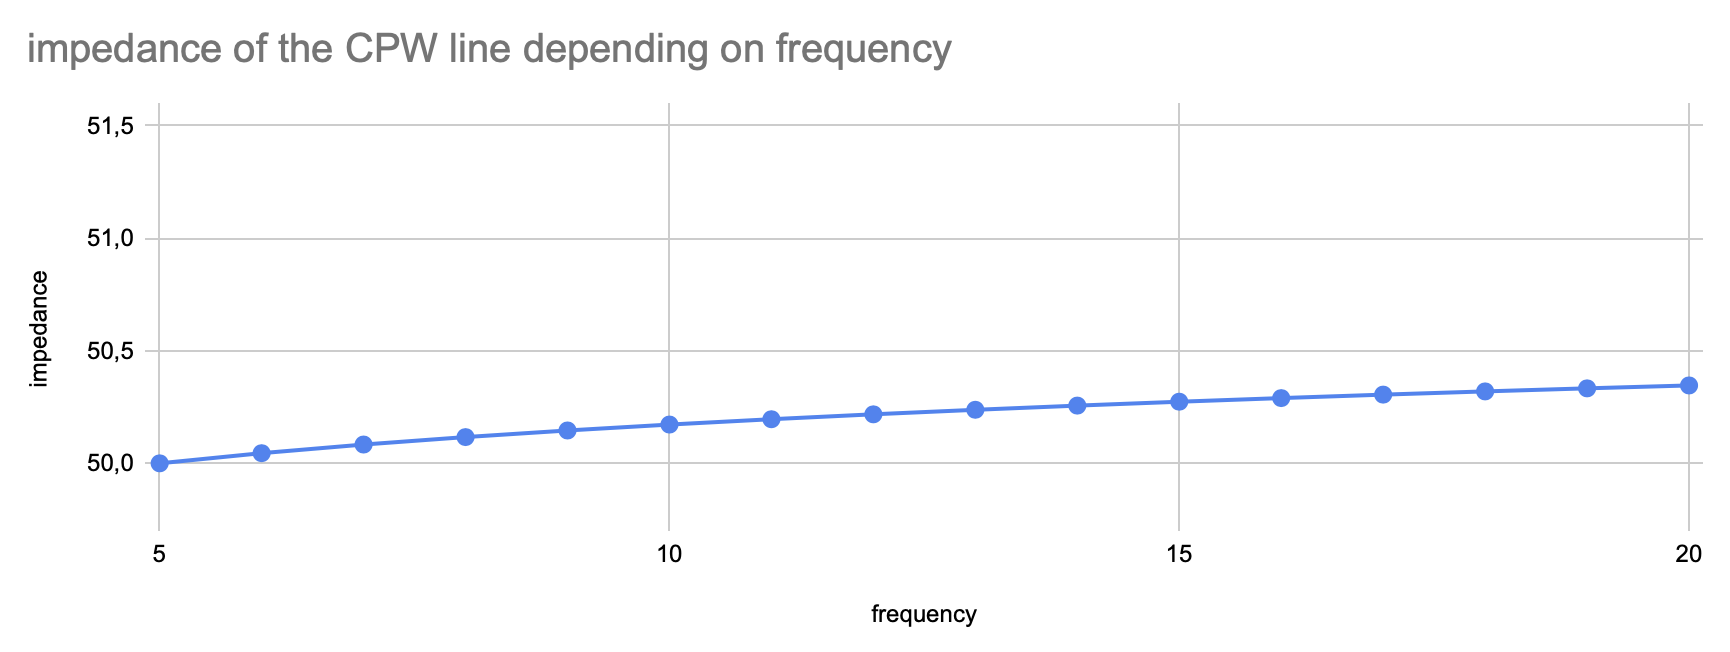
\includegraphics[width=\linewidth]{images/minitask2_impedance_vs_frequency.png}
    \caption{$Z_0$ versus frequency (5--20 GHz).}
    \label{fig:zo_freq_cpw}
\end{figure}

The results show that $Z_0$ increases very slightly with frequency: from exactly 50~$\Omega$ at 5 GHz up to 50.35~$\Omega$ at 20 GHz. 
This is a total change of only about 0.35~$\Omega$ over the whole range. The reference value of 50~$\Omega$ is found at the target design frequency of 5 GHz. 
This tiny change shows that frequency has a \textbf{limited effect} on $Z_0$ for this CPW configuration.

\subsection{B. Effect of Substrate Parameters on $Z_0$}

\subsubsection{Relative Permittivity $\varepsilon_r$}

$\varepsilon_r$ is varied from 1.4 to 7.4 in steps of 1, with all other parameters kept at their reference values.

\begin{figure}[h]
    \centering
    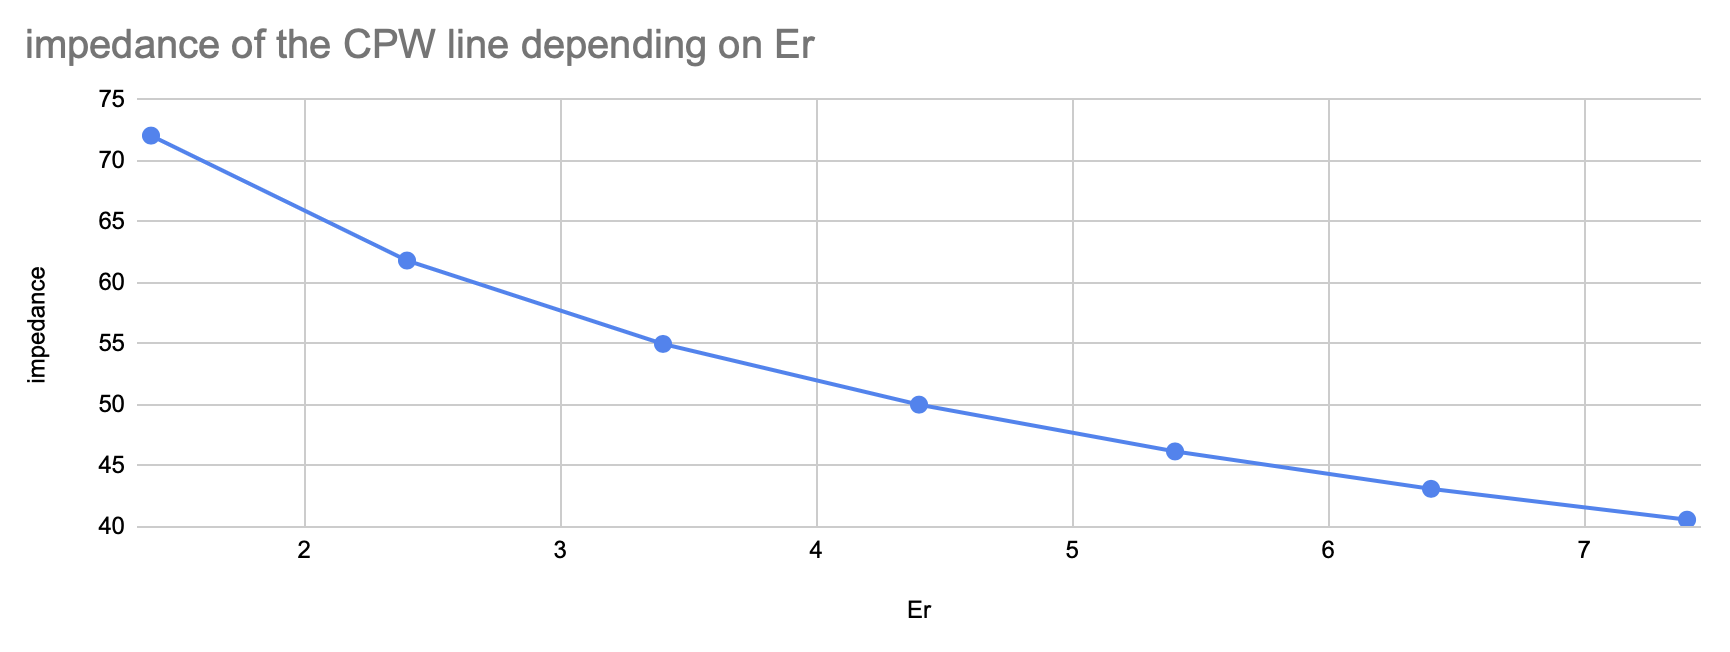
\includegraphics[width=\linewidth]{images/minitask2_impedance_vs_permittivity.png}
    \caption{$Z_0$ versus $\varepsilon_r$.}
    \label{fig:zo_er_cpw}
\end{figure}

The results show a clear \textbf{decreasing} relationship between $\varepsilon_r$ and $Z_0$ : 
from 72.03~$\Omega$ at $\varepsilon_r$=1.4 down to 40.58~$\Omega$ at $\varepsilon_r$=7.4. 
This is a total change of about 31.45~$\Omega$. The reference value of 50~$\Omega$ is found exactly at $\varepsilon_r$=4.4, 
which matches the FR4 substrate design target. Just like with the microstrip line, a higher permittivity increases the 
capacitance of the line, which lowers $Z_0$. The relative permittivity is a \textbf{significant} parameter.


\subsubsection{Loss Tangent $\tan\delta$}

$\tan\delta$ is varied from 0.01 to 0.05 in steps of 0.01.

\begin{figure}[h]
    \centering
    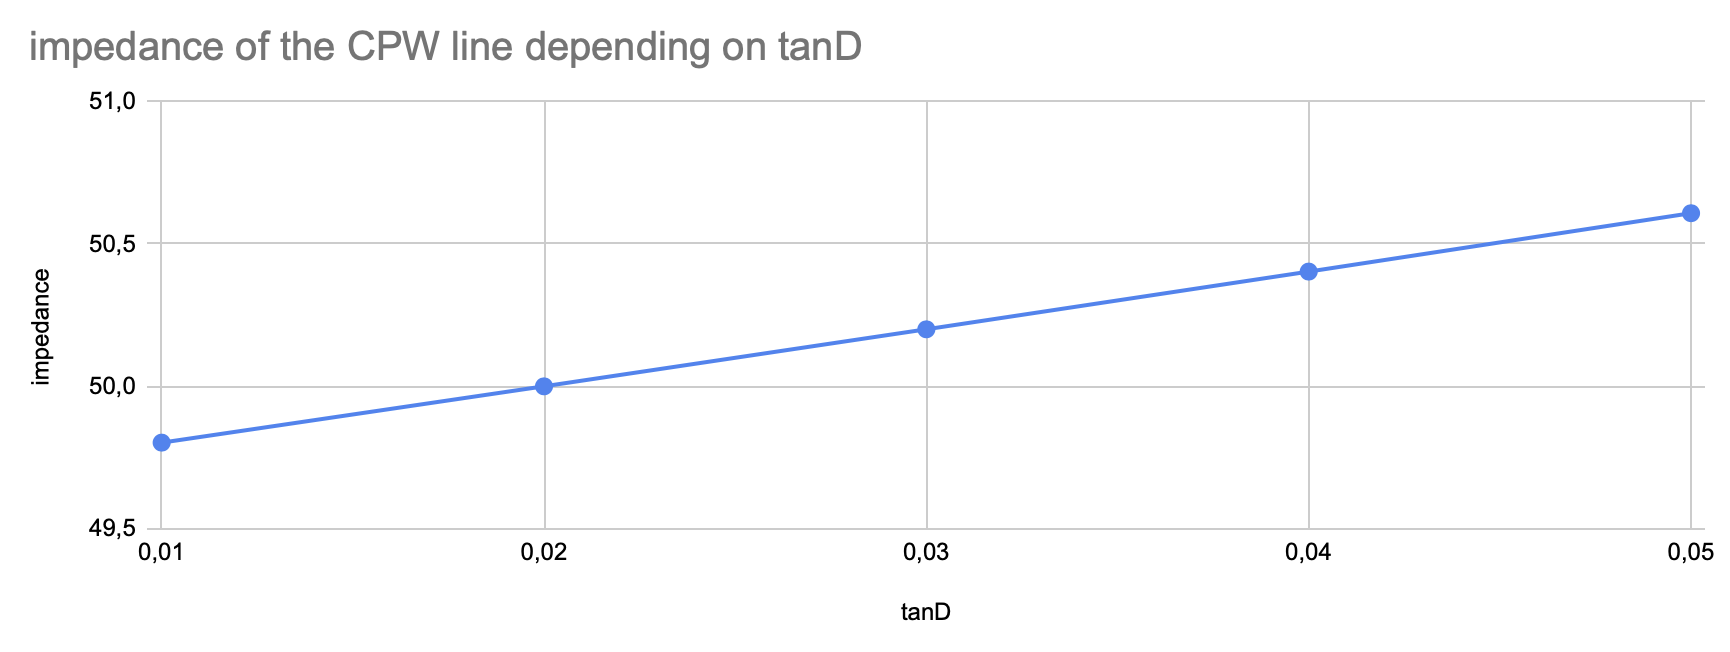
\includegraphics[width=\linewidth]{images/minitask2_impedance_vs_tanD.png}
    \caption{$Z_0$ versus $\tan\delta$.}
    \label{fig:zo_tand_cpw}
\end{figure}

$Z_0$ goes from 49.80~$\Omega$ at $\tan\delta$=0.01 up to 50.61~$\Omega$ at $\tan\delta$=0.05. 
This is a very small change of about 0.81~$\Omega$ over the tested range. This confirms that $\tan\delta$ 
has a \textbf{negligible effect} on the characteristic impedance.

\subsubsection{Substrate Thickness $H$}

H is varied from 0.1 mm to 1 mm in steps of 0.1 mm.

\begin{figure}[h]
    \centering
    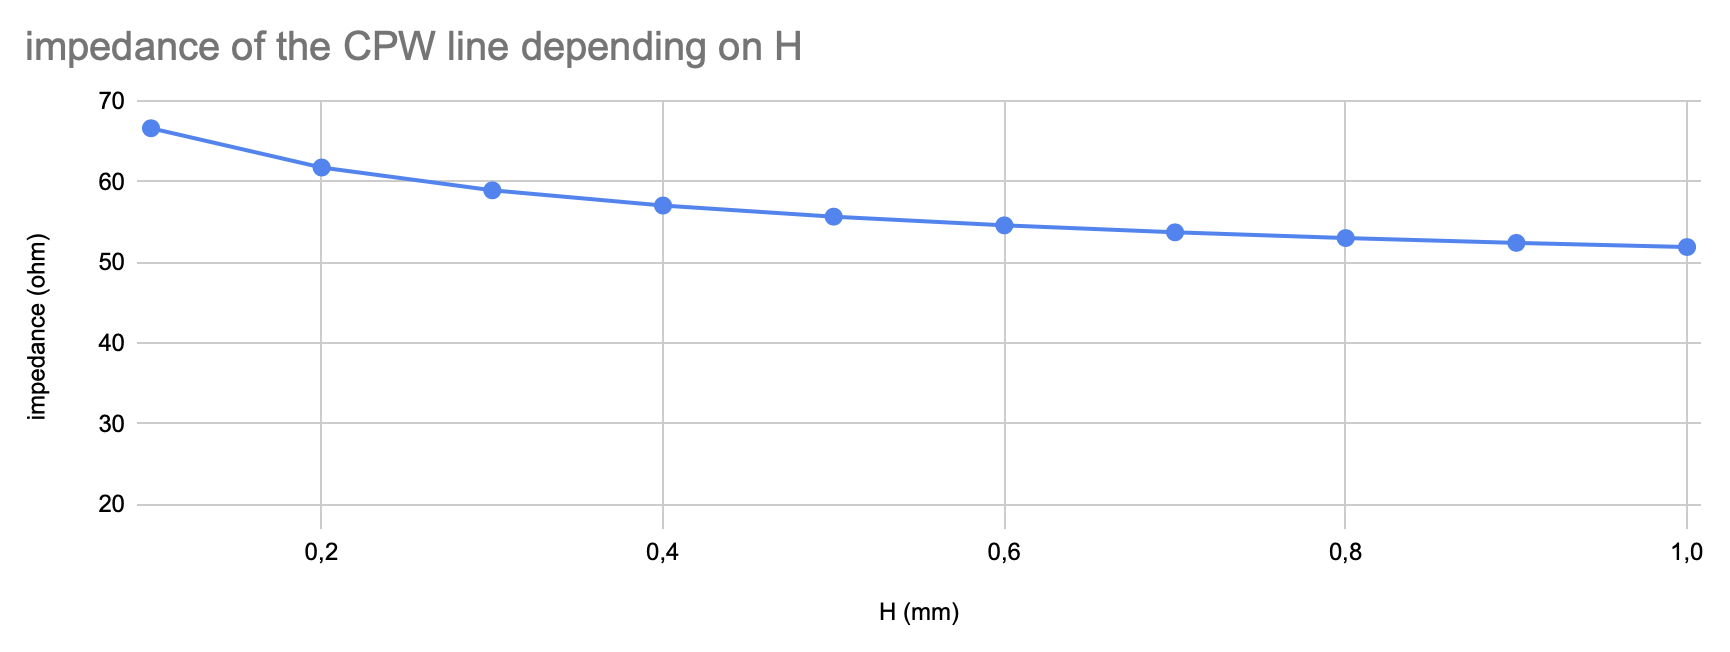
\includegraphics[width=\linewidth]{images/minitask2_impedance_vs_H.png}
    \caption{$Z_0$ versus substrate thickness $H$.}
    \label{fig:zo_H_cpw}
\end{figure}

As H increases, $Z_0$ drops from 66.66~$\Omega$ at H=0.1 mm down to 51.93~$\Omega$ at H=1 mm. 
This is a total change of about 14.73~$\Omega$. This shows a \textbf{decreasing and non-linear} 
relationship. In a CPW, a thicker substrate means more of the electric field lines are concentrated 
inside the dielectric material rather than the air, which increases the effective capacitance and 
lowers the impedance. Substrate thickness has a \textbf{moderate} effect on $Z_0$.

\subsection{C. Effect of the Line's Physical Parameters on $Z_0$}

\subsubsection{Conductor Width $W$}

W is varied from 0.1 mm to 1 mm in steps of 0.1 mm.

\begin{figure}[h]
    \centering
    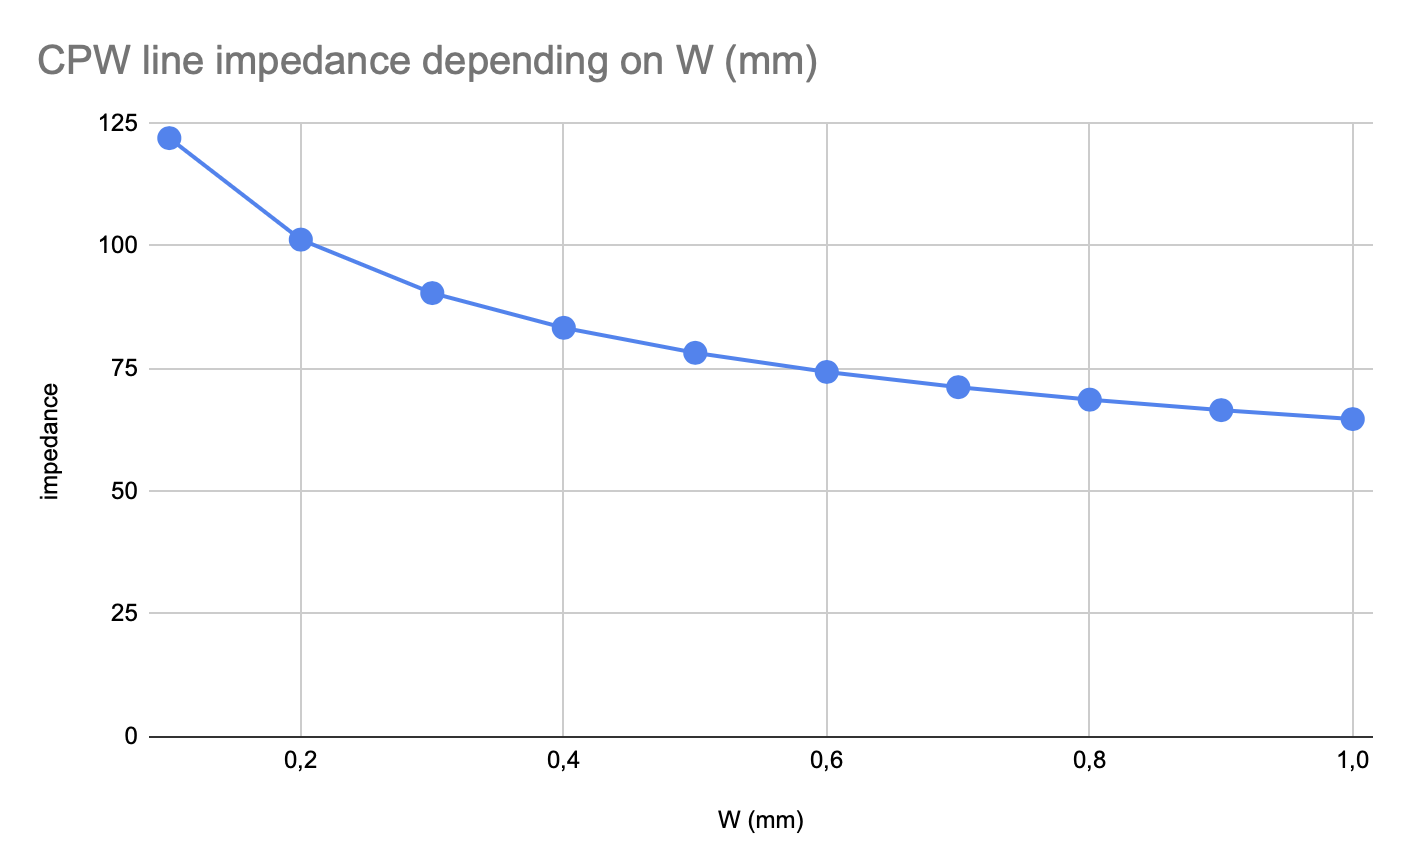
\includegraphics[width=\linewidth]{images/minitask2_impedance_vs_W.png}
    \caption{$Z_0$ versus conductor width $W$.}
    \label{fig:zo_W_cpw}
\end{figure}

$Z_0$ drops strongly as W increases: from 121.95~$\Omega$ at W=0.1 mm down to 64.65~$\Omega$ at W=1 mm. 
This is a massive change of about 57.30~$\Omega$. The relationship is \textbf{decreasing and non-linear}. 
A wider center conductor increases the capacitance, which lowers $Z_0$. The width W is a \textbf{dominant} physical parameter.

\subsubsection{Gap Width $G$}

G is varied from 0.05 mm to 1 mm in steps of 0.05 mm.

\begin{figure}[h]
    \centering
    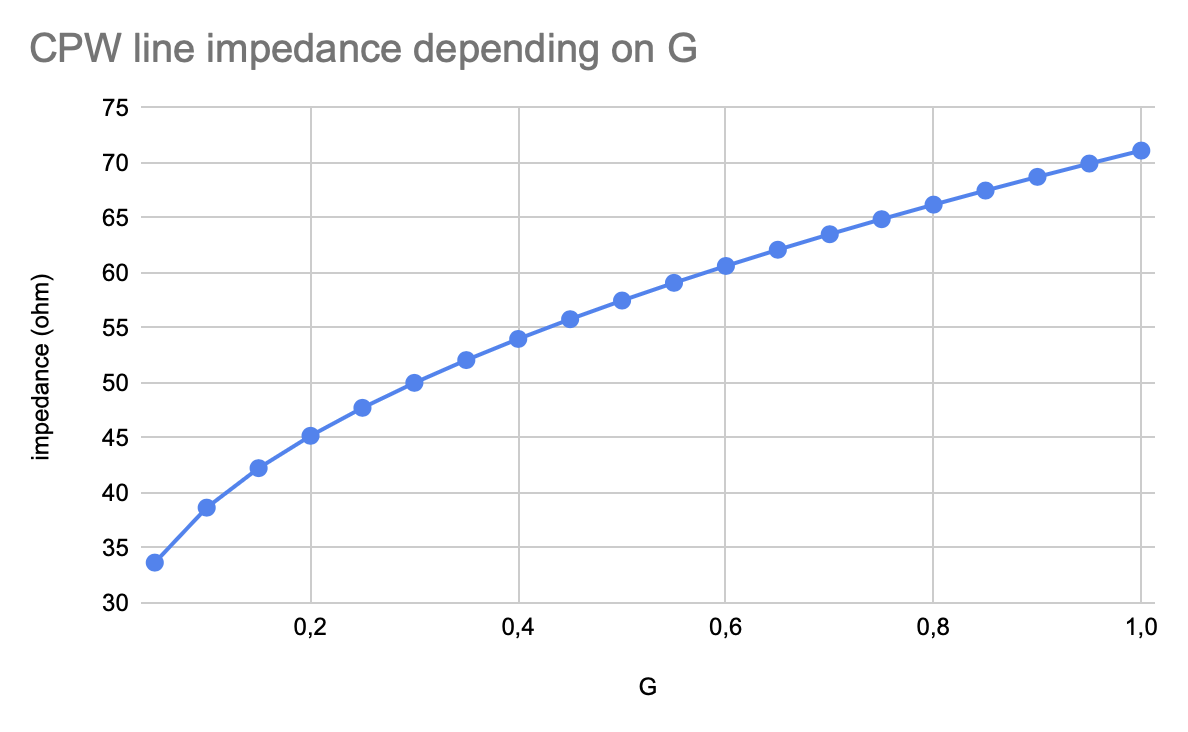
\includegraphics[width=\linewidth]{images/minitask2_impedance_vs_G.png}
    \caption{$Z_0$ versus gap width $G$.}
    \label{fig:zo_G_cpw}
\end{figure}

As the gap G between the center conductor and the ground planes gets larger, $Z_0$ 
increases steadily from 33.66~$\Omega$ at G=0.05 mm up to 71.11~$\Omega$ at G=1 mm. 
This is a total change of about 37.45~$\Omega$. The relationship is \textbf{increasing and non-linear}. 
A wider gap reduces the capacitive coupling between the center trace and the grounds, which raises the 
impedance. The gap G is also a \textbf{dominant} parameter for CPW lines.

\subsubsection{Line Length $L$}

L is varied from 10 mm to 100 mm in steps of 10 mm.

\begin{figure}[h]
    \centering
    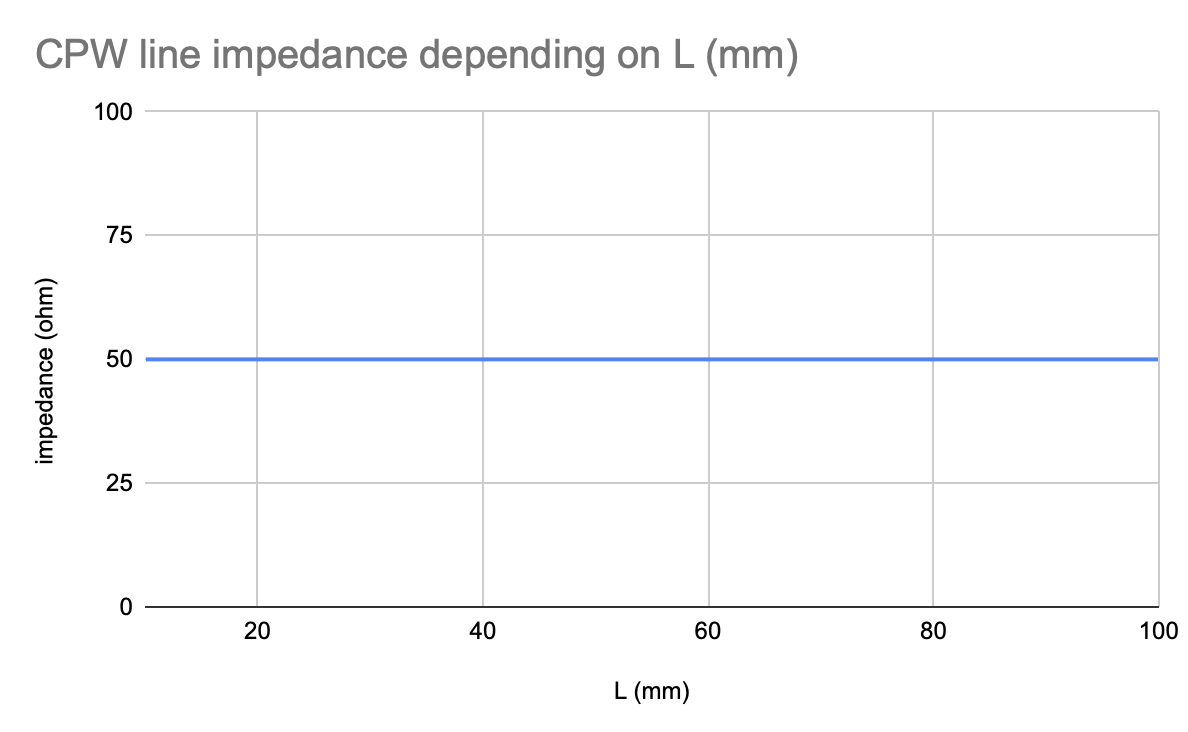
\includegraphics[width=\linewidth]{images/minitask2_impedance_vs_L.png}
    \caption{$Z_0$ versus line length $L$.}
    \label{fig:zo_L_cpw}
\end{figure}

$Z_0$ stays \textbf{perfectly constant} at 50~$\Omega$ for every value of L tested. 
Just like with the microstrip line, the length L only affects the phase shift (electrical length), but has \textbf{no effect} on $Z_0$.

\subsection{Conclusion of Mini-Task 2}

\begin{table}[h]
\centering
\begin{tabular}{lcc}
\hline
\textbf{Parameter} & \textbf{$Z_0$ range obtained} & \textbf{Effect on $Z_0$} \\
\hline
Frequency (5--20 GHz)      & 50.00 -- 50.35~$\Omega$ & Small        \\
$\varepsilon_r$ (1.4--7.4) & 40.58 -- 72.03~$\Omega$ & Significant  \\
$\tan\delta$ (0.01--0.05)  & 49.80 -- 50.61~$\Omega$ & Negligible   \\
H (0.1--1 mm)            & 51.93 -- 66.66~$\Omega$ & Moderate     \\
W (0.1--1 mm)            & 64.65 -- 121.95~$\Omega$ & Dominant     \\
G (0.05--1 mm)           & 33.66 -- 71.11~$\Omega$ & Dominant     \\
L (10--100 mm)           & 50~$\Omega$ (constant)  & None         \\
\hline
\end{tabular}
\caption{Summary of the effect of each parameter on $Z_0$ for the CPW line.}
\label{tab:synthese_minitask2}
\end{table}